%!TEX root = thesis_main.tex

\chapter{Introduction}\label{ch:intro}
Robotic systems often demand high reduction drives in small packages for use in robotic manipulators, vehicles, and many other applications. There are many choices for these reductions: planetary gearsets, belt drives, and harmonic drives. Harmonic drives, outlined in section \ref{intro:harmonic}, are the usual go-to reduction when a compact design with high reduction is needed. However, these drives cannot be custom manufactured easily and have torque limitations due to their design. Cycloidal transmissions, outlined in section \ref{intro:cycloid} are an alternative high-reduction actuator style that can achieve a high reduction in compact packages and carry substantially more torque per mass. Following the overview of these two types of reductions is a summary of the contributions of this thesis (Section \ref{intro:contribution}) and an outline of the remaining chapters of the work (Section \ref{intro:outline}). 

\section{Motivation} \label{intro:motivation}

As robotic applications flourish in our modern world, robotic systems are being pushed to be smaller, lighter, and more efficient. 
Therefore, the need for effective torque reduction in small, compact, and weight efficient packages increases. 
The prevalence of robots in development throughout the world is striking. 
Many will recognize the famous robots like the great robots out of Boston Dynamics such as Big Dog, Atlas, Spot, and many others, or the Honda's Asimo \cite{ref:asimo}.
However, this is a very small subset of the robots that are currently on the market now. 
There are a huge number of 6 DoF manipulators being constructed and sold including the UR series from Universal Robotics, the industrial arms from KUKA, ABB, Fanuc, DENSO, and even small servo operated arms available for hobbyists. 
Nearly every one of these larger robots has some sort of gear reduction between the motor and the output of each joint. Therefore, the needed expansion of available technologies for these reductions is clear as robotics push further and further into our factories, cities, and everyday lives. 

\begin{figure}[!b]
   \centering
   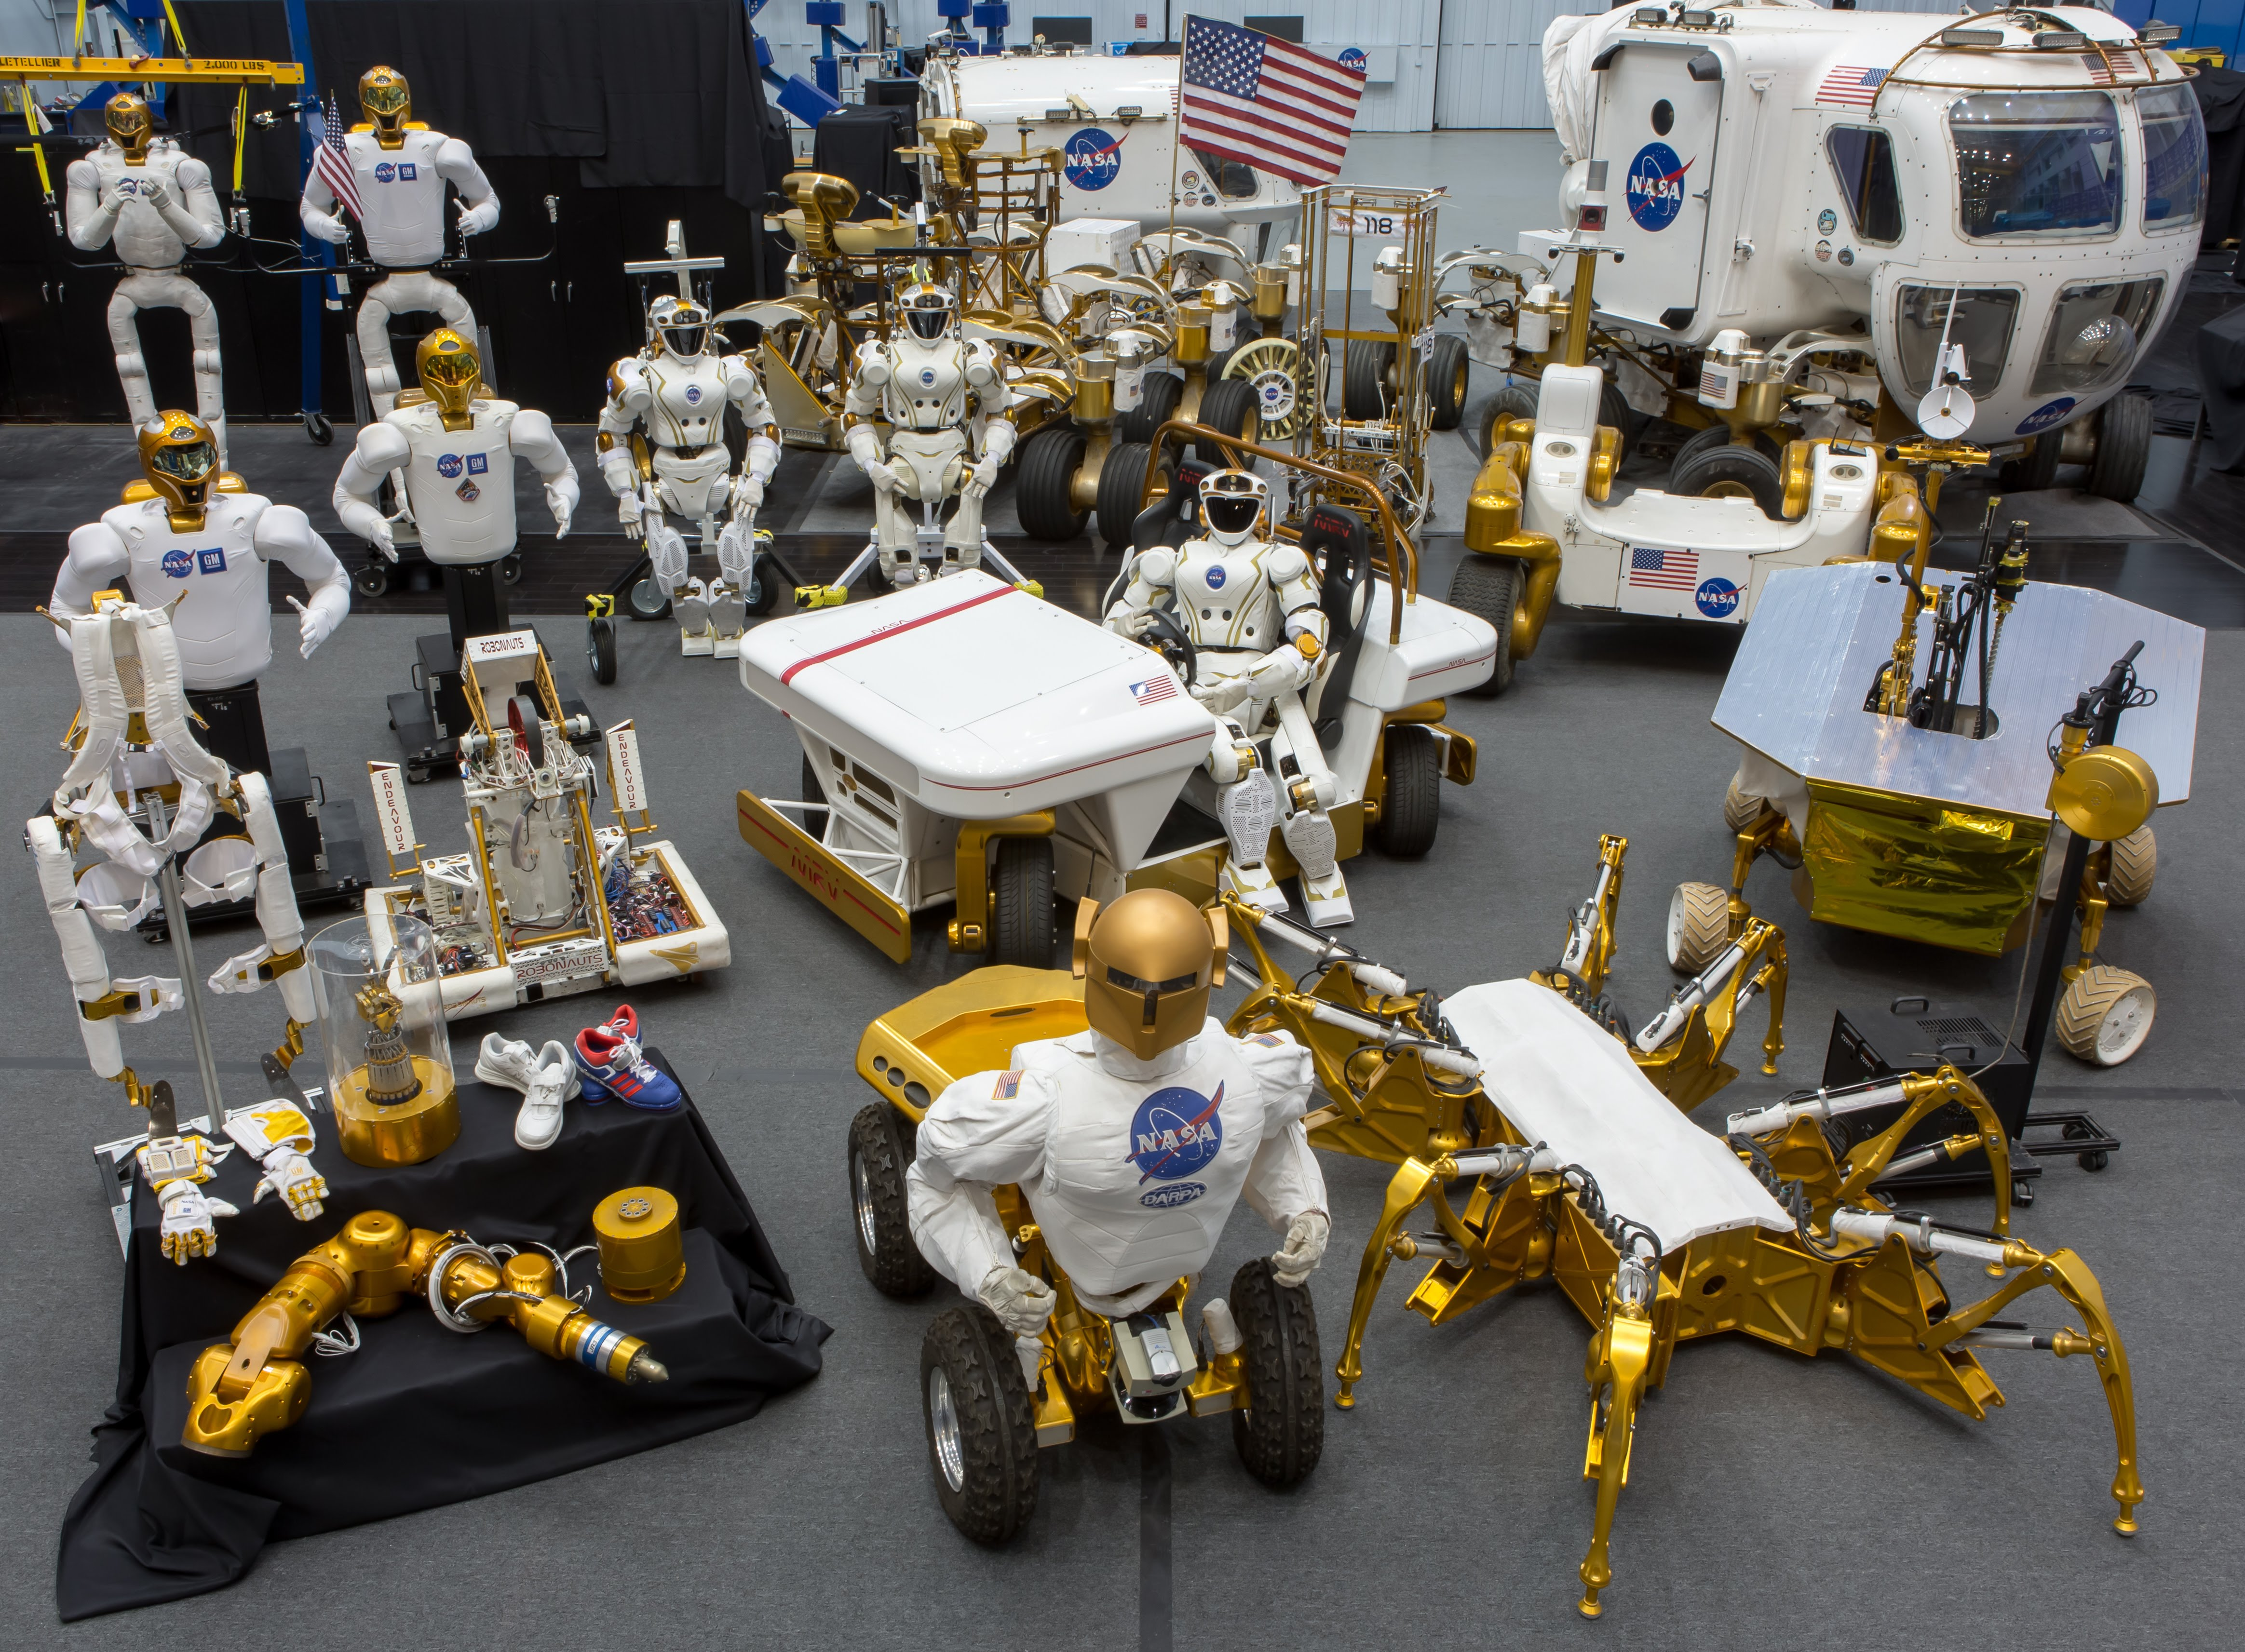
\includegraphics[width=0.7\linewidth]{fig/robot_collage}
   \caption{The family of NASA, Johnson Space Center, robots including both humanoid and mobile platforms}
   \label{fig/robot_collage}
\end{figure}

These technologies also translate directly to the work being done by NASA in the area of robotics. 
NASA is active in many types of robotic systems including humanoid robotics, rovers, and satellite technologies. 
Two quintessential examples of NASA's robotic technologies come from their humanoid robots, Robonaut 2 (R2) \cite{ref:r2}, and Valkyrie \cite{ref:valkyrie}, and the rover technologies like the Mars rovers, including the most recent rover, Curiosity \cite{ref:curiosity}, as well as the manned rover prototypes \cite{ref:rover} and lunar rovers \cite{ref:RP}.
These robotic systems share many of the same design challenges as those found in industry, as well as additional challenges due to the extreme environments in which they operate. The advancement of actuator technology is especially important in these areas as NASA strives to explore farther out into the solar system with both humans and robotic systems. 

These robots must balance a number of factors based on their specific design goals, which usually involve efficiency, strength, speed, and precision in some combination. 
In combination with these aforementioned goals is the trade of the actuator design factors such as backlash, backdriveability, efficiency, torque output, speed, and size. 
Reductions for these systems can be broadly generalized into one of three types: planetary gearsets, belt drives, and harmonic drives. 
Each of these drives has their own advantages. 
Planetary gearsets can be customized to meet a desired reduction, are commonly produced, and run very efficiently.
Belt drives share many of the benefits of planetary gearsets and have very minimal backlash, but require more volume for a similar reduction. 
Harmonic drives are generally much more compact for the reduction they provide and have no backlash as well, but run less efficiently than the other two. 
Due to their higher reduction per volume, harmonic drives are a common reduction of choice in robotic actuator design when compact design is favored over efficiency.

There exists a fourth option to add to this list, cycloidal drives. 
Cycloidal drives provide a high reduction per volume, similar to a harmonic drive, but can provide a higher specific torque than a harmonic drive. 
Cycloidal drives generally do have backlash, so they cannot replace a harmonic drive in every situation. A cycloidal drive provides an interesting option in design cases where high reduction and high torque in a small package are necessary and a small amount of backlash is acceptable. 
However, even with these distinct advantages over a harmonic drive, these cycloidal drives are not currently in common use partially due to the lack of information on their actual in-use characteristics. 

\section{Harmonic Drives} \label{intro:harmonic}

The concept of a harmonic drive was proposed as early as 1959 by Walton Musser \cite{ref:harmonic_original} and have been further improved in design and implementation through the years. The original harmonic drive patent has been cited in over 200 subsequent patents according to Google patent search. These drives were first used in spaceflight applications in 1971 as the primary drive motors for the Apollo Lunar Rovers \cite{ref:harmonic_apollo}. A notable adaptation of this patent led to the current common method of manufacturing harmonic drives. This patent issued to Harmonic Drive in 1989 \cite{ref:harmonic_drive_co} making the Harmonic Drive company one of the primary producers of harmonic drive technologies until recently when the patent expired. 

Harmonic drives utilizes the deflection of metal to induce motion. These drives consist of three main pieces: a wave-generator, a flex cup, and a circular spline (Fig \ref{fig:harmonic_cartoon}). The wave generator is a slightly elliptical shape which is mounted to the output of the motor. This is inserted into the flex cup, a thin metal cup with \textit{N\textsubscript{flex}} teeth that allows some flexing as the elliptical wave-generator rotates through it. Finally, the flex cup and wave-generator system are inserted into the circular spline which is a thicker, stiff piece of metal that has a different number of teeth, \textit{N\textsubscript{circ}}, (typically 1 more tooth) than the flex cup. As the wave-generator rotates inside the flex cup, pushing the walls out, it slowly works its way into the next available tooth, creating a counter-rotation of the flex-cup, which is harnessed as the output of the system. This results in high ratios in the form of 

\begin{equation} \label{eq:harmonic_ratio}
ratio = \frac{N_{flex} - N_{circ}} {N_{flex}}.
\end{equation}

\begin{figure}[t]
   \centering
   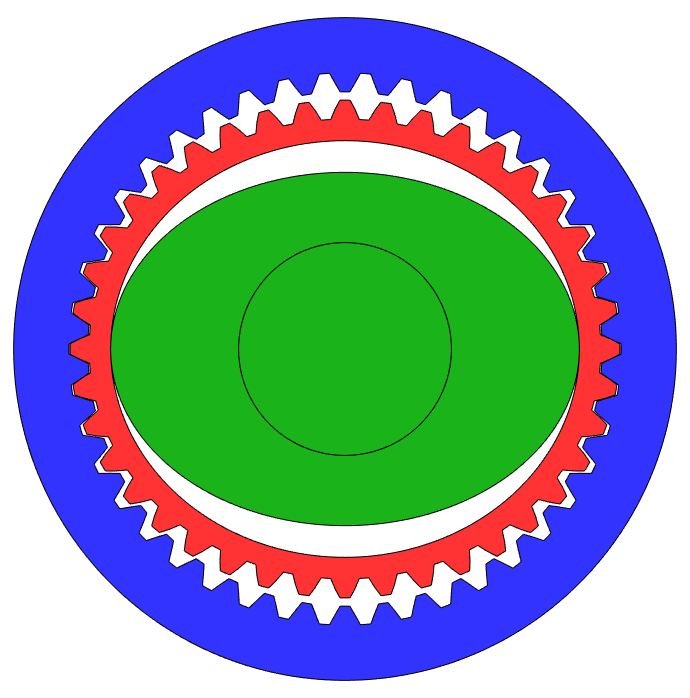
\includegraphics[width=0.3\linewidth]{fig/harmonic_blank}
   \caption{Cartoon rendering of the primary components of a harmonic drive, the wave-generator (green), flex-cup (red), and the circular spline (blue). The wave-generator is connected to the input shaft, the circular spline is fixed to the housing, and the output is harnessed through the motion of the flex-cup. (Public domain figure from \cite{ref:harmonic_cartoon})}
   \label{fig:harmonic_cartoon}
\end{figure}

Harmonic drives have two primary advantages in their use. First, harmonic drives can accomplish high reductions in a smaller volume than a typical planetary reduction. Second, harmonic drives have no backlash, allowing precision control with no additional considerations required. However, these advantages come with a cost. The efficiency of harmonic drives is generally substantially lower than their planetary counterpart and varies drastically with temperature. In Figure \ref{fig:harmonic_eff} a reproduction of the efficiencies quoted in the harmonic drive manual \cite{ref:harmonic_sheet} can be seen for reference. These efficiency results can be further supported for space applications by the research of Schafer et. al. \cite{ref:harmonic_space_lube} and \cite{ref:harmonic_performance}. Even with these disadvantages, harmonic drives are still the primary source of high reduction ratios in robotic platforms today. 

\begin{figure}[t]
   \centering
   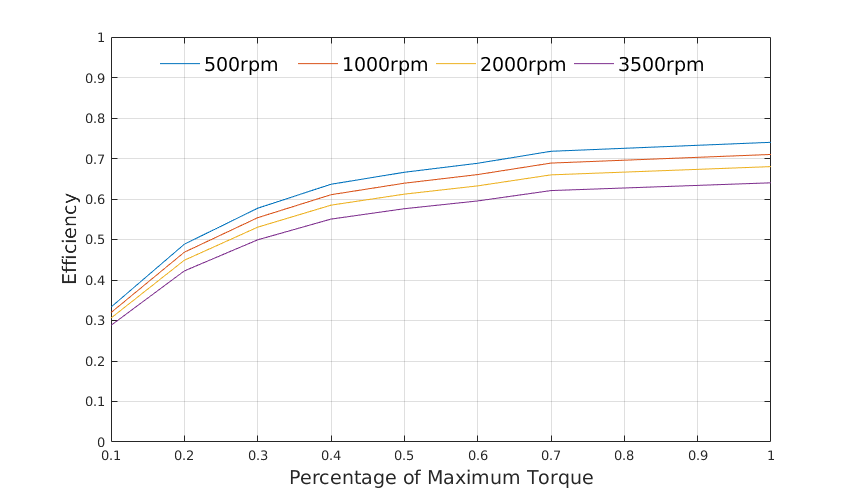
\includegraphics[width=0.9\linewidth]{fig/harmonic_eff}
   \caption{Harmonic efficiencies over the torque input for a Harmonic Drive CSF-45-50-2UH-LW, which is a similarly sized actuator to the single-stage cycloidal drive studied in this work.}
   \label{fig:harmonic_eff}
\end{figure}

\section{Cycloidal Drives} \label{intro:cycloid}

An alternative technology for high reductions in small packages comes in the form of cycloidal drives and is the primary focus of this work. The original concept for the induced motion seen in a cycloidal drive pre-dates harmonic drive. The original patent for the motion of the cycloid was filed by James Johnson in 1931 \cite{ref:cycloid_original}. However, the development of this technology did not accelerate at the same speed as the harmonic drive, this original patent only received 12 citations. A major advancement in the technology came when Rudolf Braren proposed in 1977 the concept and equations necessary for the common method of constructing cycloids that is used today.\cite{ref:cycloid_one_stage}. In 1981, Keith Rodaway patented the concept of a pinwheel reduction \cite{ref:cycloid_pinwheel}, which allowed much more compact designs of the cycloidal system. The invention of this compact design style is the premise for the compact, high torque density, and high specific torque designs that are discussed in this work.

The premise of this design leverages a plate, referred to as the cycloid plate, with lobes that interact with pins in the housing being spun on an eccentric shaft with a bearing.
The interaction between the eccentric rotation and the lobes pressing between the pins induces a counter-clockwise motion of the plate. This counter-clockwise rotation is harnessed via the interior pins that connect to a concentric plate that acts as the output of the mechanism (seen in Fig \ref{fig:cycloid_cartoon}). The reduction equation \ref{eq:single_stage_ratio} gives the overall reduction of the single-stage cycloid where \textit{N\textsubscript{lobes}} is the number of lobes on the cycloid plate and \textit{N\textsubscript{pins}} is the number of pins in the housing. 

\begin{equation} \label{eq:single_stage_ratio}
Q = \frac{N_{lobes}} {N_{pins} - N_{lobes}}
\end{equation}

\begin{figure}[t]
   \centering
   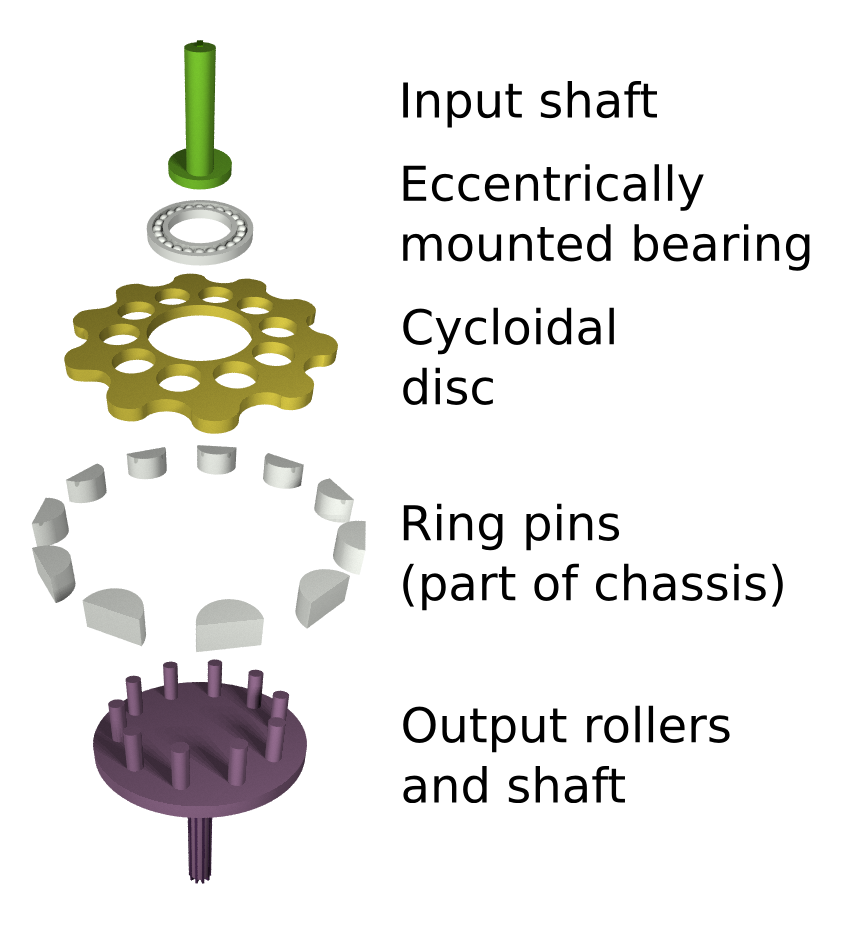
\includegraphics[width=0.40\linewidth]{fig/Cycloidal_drive_parts}
   \caption{Simple rendering of the key elements that create a cycloidal drive.
   A drive shaft spins a cycloidal disk via an eccentric circle (green).
   The cycloid plate (yellow) reacts against the housing pins (gray) to create a counter-rotation, harnessed by the output pins (purple). (Public domain image from \cite{ref:cycloid_cartoon})}
   \label{fig:cycloid_cartoon}
\end{figure}

This geartrain design has been used for industrial applications orr high torque, high shock load systems for many years, including companies like Natbesco Motion Control and Onvio. The mechanics of the design allow for large shock loads to pass through the system since most of the components are solid pieces of metal that can deflect into each other to share the load. 
However, in many of these applications, many or all of the interacting surfaces, like the housing pins and output pins, use needle roller bearings to transmit load.
This allows for higher efficiency and load carrying capability, but, also increases mass and volume.
In the robotic industry, groups are striving to reduce the mass and volume of these actuators, while still achieving high reduction and load capabilities.
One method for reducing mass is eliminating the roller bearings at the interaction points between the cycloid plate, housing pins, and output pins.
This allows for very compact and strong designs to be considered, but it leaves the potential for larger losses and shorter system lifetimes. The details of this design will be presented in Chapter \ref{ch:design_1s} and the efficiency of an example compact design will be presented in Chapter \ref{ch:dual}. 

Many works have been presented on the subject of the theoretical design of these cycloidal drives \cite{ref:on_the_lobe} \cite{ref:hwang_hsieh}, designing with machine tolerances \cite{ref:design_and_application}, contact and stress analysis \cite{ref:li}, and performance characteristics, such as torque ripple and backlash \cite{ref:hsieh_traditional} \cite{ref:hsieh_dynamics}, These topics will be discussed further in Chapter \ref{ch:design_1s}.
These works lay a solid foundation for a designer, providing the equations and design considerations for a single-stage cycloid. There is even work outlining the use of genetic algorithms for the theoretical sizing of the actuators \cite{ref:single_genetic}.
Still, there is a need to present in-use characteristics to support the theoretical calculations and models.

Theoretical cycloid efficiencies have been reported to be in the 88-98\% range \cite{ref:malhorta_2}, \cite{ref:unified_approach}.
More recently, Sinsinger and Lipsey reported experimentally determined efficiencies for fused roller designs (42.3\%) and pin designs (71\%) based on 80 minutes of run-time \cite{ref:cycloid_vs_harmonic}.
The distinction between a fused roller and a pin design is in the design of the housing.
In a fused design, the input pins are machined as part of the housing. 
In a pin design, pins are inserted to ride in channels cut in the housing, allowing relative motion between the pin and the housing.

Hsieh verified the stress present in the drives in both simulation and an in-use application which demonstrated lower stress levels and torque ripple when using fused rollers \cite{ref:hsieh_dynamics}.
These two results leave an open trade to designers if stress and torque ripple need to be minimized versus maximizing efficiency.

More recently, authors have proposed designs that create a ``two-stage'' reduction using the cycloid profile. In a typical two-stage reduction, the output of the first reducer is used as the input of the second reducer. Instead, for a two-stage cycloid, the counter-rotation and wobble of the first stage is passed to a second cycloid plate. This second cycloid plate, with a different number of lobes from the first, interacts with a set of housing pins that is free to rotate \cite{ref:new_two_stage}. This design allows for more compact high reduction systems with a reduction defined in eq. \ref{eq:two_stage_ratio} \cite{ref:two_stage_tooth_mod} with \textit{N\textsubscript{1}} stage 1 pins and \textit{N\textsubscript{2}} stage 2 pins with a single tooth difference in each. The details of this design with be outlined more completely in Chapter \ref{ch:dual}.

%put 2 stage equation
\begin{equation} \label{eq:two_stage_ratio}
Q = \frac{1}{1 - \frac{N_1 (N_2-1)}{N_2 (N_1-1)}}
\end{equation}

The previous work in this area lays a foundation of understanding for the construction and theoretical design of a single-stage cycloidal drive. However, there is a gap in the literature when it comes to in-use efficiency and lifetime of these devices. The benefits of designs like this are clear, but under-utilized in the robotic community. Additionally, the concept for a two-stage cycloid has been presented, but, is lacking in some of the necessary design equations to produce compact two-stage cycloids. 

\section{Contribution} \label{intro:contribution}

The contributions of this thesis is three-fold,
\begin{enumerate}
	\item Development of explicit relative velocity equations for the lobe to pin interaction of a single-stage cycloid, further developing predicted loss equations.
	\item Long duration testing of a compact pin-in-housing single-stage cycloid reducer.
	\item Development of force and velocity equations for a fused two-stage cycloid, yielding predicted loss equations. 
\end{enumerate}
Through these three items, key gaps in the literature are closed. First, a closed form solution for the relative motion between lobes and pins has yet to be presented, allowing estimated losses for this interaction. Second, very limited testing has been presented for a compact, pin-in-housing design of a single-stage cycloid. Therefore, extended duration testing is presented to understand in-use efficiency and lifetime for these actuators. Finally, very little has been presented on the new two-stage cycloid design aside from the geometric analysis, so, closed form solutions for velocity and force for the lobe to pin interactions is developed to give predicted losses for a two-stage design. These losses are compared to a two-stage test article. This leads to recommendations that can be made for future designers of these devices. 

\section{Thesis Outline} \label{intro:outline}
The body of this thesis is broken into three chapters. Chapter 2 will cover the design equations for a single-stage cycloid, the design of the tested single-stage drive, and the development of closed form equations for the relative velocity between the lobes and rollers of a single-stage cycloid. Chapter 3 will discuss the testing procedure and results for the single-stage cycloid that was tested. Chapter 4 will then cover the design equations present in the literature for a new two-stage cycloid and build upon this literature to discuss the relative velocity between the pins and lobes, forces present in these interactions, and the predicted losses. This is compared to the constructed two-stage cycloid to give a ground truth for the analysis. Design recommendations are then presented stemming from the results of this analysis. Finally, Chapter 5 will summarize the results and conclusions of this work. 

